	\documentclass[]{beamer}
	\usepackage[latin1]{inputenc}
	\usepackage{textpos}
	\usepackage{graphics}
	\usepackage[english]{babel}
	\usepackage{colortbl}
	\usepackage{caption}
	% \usepackage{subcaption}
	\usepackage{multirow}
	\usepackage{amsmath}
	\usepackage[makeroom]{cancel}
	\usepackage{xcolor} % for colored text

	\usepackage{tikz} % for flow charts
	\usetikzlibrary{shapes,arrows,positioning,shadows,calc}

\usepackage{filecontents}% http://ctan.org/pkg/filecontents
\usepackage{silence}% http://ctan.org/pkg/silence
\WarningFilter{latex}{Overwriting file}% Remove LaTeX warnings starting with "Overwriting file"
\begin{filecontents*}{linereg.data}
#x y
0 4
10 24
\end{filecontents*} 

\begin{filecontents*}{linereg2.data}
#x y
2 8
8 20
\end{filecontents*} 

	\renewcommand<>{\item}[1]{\only#2{\beameroriginal{\item}{#1}}} % for replace a equation for other equation in the same place
	
	% \usetheme{Warsaw}
	\usetheme{Frankfurt}
	% \usetheme{Boadilla}
	\setbeamertemplate{navigation symbols}{} 
	\setbeamertemplate{mini frames}{}
	% \useoutertheme{infolines} 
\setbeamertemplate{footline}{\hbox{\vspace{0.1cm} \insertshortauthor \hspace*{3.5cm} \insertshorttitle \hspace*{4.6cm} \hfill\insertframenumber}} 

\def\braces#1{[#1]} % to define square parenthesis 
	
% \usecolortheme{orchid}

% \usecolortheme{lily}

% \usecolortheme{default}
\usecolortheme{cranejavier}



% \setbeamertemplate{footline}[frame number]
% \setbeamertemplate{footline}[page number]

% My packages
% added on 08-03-15
\usepackage[percent]{overpic}
% http://www-ljk.imag.fr/membres/Jerome.Lelong/latex/appendixnumberbeamer.sty
% Reference: http://tex.stackexchange.com/questions/2541/beamer-frame-numbering-in-appendix
\usepackage{appendixnumberbeamer}
% Add total frame count to slides, optional. From Stefan,
% http://www.latex-community.org/forum/viewtopic.php?f=4&t=2173
% \expandafter\def\expandafter\insertshorttitle\expandafter{%
%   \insertshorttitle\hfill\insertframenumber\,/\,\inserttotalframenumber}	


	
% -------------------------------------- Slide 1 -----------------
	\title[Atmospheric Correction L8]{Atmospheric Correction for Landsat 8 over Case 2 Waters}
	\author[Javier A. Concha]{\Large Javier A. Concha, John Schott\\\vspace{1cm}}
	\institute{\footnotesize Digital Imaging and Remote Sensing Lab\\Chester F. Carlson Center for Imaging Science\\ Rochester Institute of Technology}
	\date{\today}

\AtBeginSection[ ]
{	\setbeamertemplate{footline}{} 	
	\begin{frame}{\Large Atmospheric Correction for Landsat 8 over Case 2 Waters} 
	\LARGE
		\tableofcontents[currentsection]
	\end{frame}

\addtocounter{framenumber}{-1}	

\setbeamertemplate{footline}{\hbox{\vspace{0.1cm} \insertshortauthor \hspace*{3.5cm} \insertshorttitle \hspace*{4.6cm} \hfill\insertframenumber}} 
}	

% \AtBeginSubsection[ ]
% {		
% 	\begin{frame}{\LARGE Outline} 
% 		\tableofcontents[currentsection,currentsubsection]
% 	\end{frame}
% \addtocounter{framenumber}{-1}	
% }		
\newcounter{tmpc} % for resume counter
%&&&&&&&&&&&&&&&&&&&&&&&&&&&&&&&&&&&&&&&&&&&&&&&&&&&&&&&&&&&&&&&
%&&&&&&&&&&&&&&&&&&&&&&&&&&&&&&&&&&&&&&&&&&&&&&&&&&&&&&&&&&&&&&&	
	
\begin{document}
{	
\setbeamertemplate{footline}{} 
\setbeamertemplate{headline}{}
	
	\begin{frame} 
	\titlepage
	
	\begin{textblock*}{10cm}(10.0cm,-8.5cm)
	   \includegraphics[height=10mm]{/Users/javier/Desktop/Javier/MASTER_RIT/2011_THESIS/LaTeX/Presentation/tiger_walking_rit_color.eps}
	\end{textblock*}
	\begin{textblock*}{10cm}(4.7cm,-8.0cm)
	   \includegraphics[height=5mm]{/Users/javier/Desktop/Javier/PHD_RIT/ConferencesAndApplications/2014_RITResearchSymposium/Images/USGS_logo.eps}
	\end{textblock*}	
	\begin{textblock*}{10cm}(-.7cm,-8.5cm)
	   \includegraphics[height=10mm]{/Users/javier/Desktop/Javier/PHD_RIT/ConferencesAndApplications/2014_ASPRS_SOY/Images/dirs_logo.png}
	\end{textblock*}
	
	\begin{textblock*}{9cm}(2cm,-5cm)

	   \tikz\node[opacity=0.3]{ \includegraphics[width=65mm]{/Users/javier/Desktop/Javier/PHD_RIT/ConferencesAndApplications/2014_ASPRS_SOY/Images/landsat8-earth.jpg}};
	\end{textblock*}

	\begin{textblock*}{12cm}(.5cm,0cm)
	   \scriptsize Presented to: Earth Observing Systems XX Conference, SPIE San Diego, 2015 
	\end{textblock*}
	
	\end{frame}

}
\addtocounter{framenumber}{-1}
%\setbeamercovered{highly dynamic}
%\setbeamercovered{transparent}
\setbeamercovered{still covered={\opaqueness<1->{2}},again covered={\opaqueness<1->{2}}}

% ----------------------------------- Slide ----------------------------------------------	

% \addtobeamertemplate{frametitle}{}{%
% \begin{textblock*}{90mm}(8.2cm,-0.5cm)
% % \includegraphics[height=0.5cm]{/Users/javier/Desktop/Javier/MASTER_RIT/SPIE2012/Slides/rit_white_no_bar.jpg}
% \includegraphics[height=0.4cm]{/Users/javier/Desktop/Javier/PHD_RIT/ConferencesAndApplications/2014_ASPRS_SOY/Images/RIT_LOGO.png}
% \end{textblock*}}
% ----------------------------------- Slide ----------------------------------------------	
\begin{frame}{\LARGE Motivation} 
\vspace{-.5cm}
\begin{columns}[c] % contents are top vertically aligned
  	\begin{column}[T]{6cm} % each column can also be its own environment
  		\vspace{0.5cm}
      	\begin{itemize}
      	\Large
      		\item Ocean Color Satellites (e.g. MODIS, SeaWiFS): \\ \LARGE Global Studies
      	\end{itemize}
	\end{column}

  	\begin{column}[T]{6cm} % each column can also be its own environment
 		\begin{figure}[H]
 			\includegraphics[height=3cm]{/Users/javier/Desktop/Javier/PHD_RIT/ConferencesAndApplications/2014_ASPRS_SOY/Images/107325main_chloro_concentrate.jpg}
 		\end{figure}
 		\vspace{-0.7cm}
 		{\hspace{4.2cm}\tiny $*~$Credit: NASA}
 	\end{column}
\end{columns}

\begin{figure}[H]
		\includegraphics[height=4cm]{/Users/javier/Desktop/Javier/PHD_RIT/ConferencesAndApplications/2014_ASPRS_SOY/Images/DiffResol.png}
\end{figure}
\end{frame}
% ----------------------------------- Slide ----------------------------------------------
{
\setbeamertemplate{footline}{} 
\begin{frame}{\Large Atmospheric Correction for Landsat 8 over Case 2 Waters} 
\LARGE
	\tableofcontents
\end{frame}

\addtocounter{framenumber}{-1}
}

%%%%%%%%%%%%%%%%%%%%%%%%%%%%%%%%%%%%%%%%%%%%%%%%%%%%%%%%%%%%%%%%%%%%%%%%%%%%%%%%%%%%%%%%%%
\section{Goal}
\subsection*{Goal}
% ----------------------------------- Slide ----------------------------------------------
\begin{frame}{\LARGE Big Picture} 
\begin{itemize}
\LARGE

\item To Use Landsat 8 to retrieve Color Producing Agents (CPAs):
\begin{itemize}
	\Large
 	\item chlorophyll-{\it a} ($C_a$)
 	\item colored dissolved organic matter ($CDOM$)
 	\item suspended minerals ($SM$ or $TSS$)
 \end{itemize}
\vspace{.5cm}
\item Over Coastal and Inland Water (Case 2 Waters)
\vspace{.5cm}
\item Small/Medium Scale regions

\end{itemize}

\end{frame}

% ----------------------------------------------
\begin{frame}{\LARGE Goal of this Study} 
\begin{itemize}\itemsep.5cm
\LARGE

\item To compare our atmospheric correction method with NASA's standard products
\item To compare all methods with Field Data

\end{itemize}

\end{frame}
% ----------------------------------- Slide ----------------------------------------------
\begin{frame}{\LARGE Why Atmospheric Correction is important for Water Studies?} 
 \begin{columns}[c] % contents are top vertically aligned
  	\begin{column}[T]{5cm} % each column can also be its own environment
    \includegraphics[height=5cm]{/Users/javier/Desktop/Javier/PHD_RIT/ConferencesAndApplications/2014_RITResearchSymposium/Images/SensorReachingRadiance.png}
    	    \vspace{0.2cm}
    		\centerline{Retrieved $L_w$}
     	\end{column}
  
  	\begin{column}[T]{7cm} % each column can also be its own environment
    \includegraphics[width=7cm]{/Users/javier/Desktop/Javier/PHD_RIT/ConferencesAndApplications/2014_RITResearchSymposium/Images/TOARadiance.png}
    	    \vspace{0.2cm}
    		\centerline{Retrieved $L_w$ vs $L_u$}
    		% \centerline{(Unknown concentrations)}
     	\end{column}
\end{columns}
\vspace{.5cm}
\hspace{4cm}{\scriptsize $*~$Images from: http://www.oceanopticsbook.info/}
\end{frame}

% ------------------------------ SUBSECTION ----------------------------------------------
\subsection*{Landsat 8}
% ----------------------------------- Slide ----------------------------------------------
\begin{frame}{\LARGE Why Landsat 8?} 
\vspace{-.5cm}
\begin{itemize}
\LARGE

	\item Multispectral: 4 VIS, 1 NIR, 2 SWIR
	\vspace{.2cm}
	\item Spatial resolution: 30
	\vspace{.2cm}
	\item Temporal resolution: 16 days
	\vspace{.2cm}
	\item Bit depth: 12-bits quantization (4096 levels)
	\vspace{.2cm}
	\item Pushbroom satellite
	\vspace{.2cm}
	\item Improved signal-to-noise ratio

\end{itemize}

\end{frame}
% % ----------------------------------- Slide ----------------------------------------------
% \begin{frame}{\LARGE Landsat 8} 

% \begin{figure}[H]
% 		\includegraphics[height=6cm]{/Users/javier/Desktop/Javier/PHD_RIT/ConferencesAndApplications/2014_ASPRS_SOY/Images/ldcmbands.png}
% \end{figure}

% \end{frame}
% ----------------------------------- Slide ----------------------------------------------
\begin{frame}{\LARGE Landsat 8 Image} 


\begin{figure}[htb]
  \begin{minipage}[c]{0.6\linewidth}
    \centering
      \includegraphics[trim=0 0 0 0,clip,height=6.5cm]{/Users/javier/Desktop/Javier/PHD_RIT/Latex/Proposal/Images/groundtruth-sitenames-no-ends.jpg}  
  \end{minipage}
  \hfill
  \begin{minipage}[d]{0.3\linewidth}
    \centering
      \includegraphics[trim=0 0 0 0,clip,height=3cm,angle=90]{./Images/JavierSampling.JPG}
  \end{minipage}
  % \caption{PIF mask determination. (a) False color image, with vegetation in red and (b) PIF mask over downtown Rochester. \label{fig:PIFmask} } 
\end{figure}

% \begin{figure}[htb]
%   \centering
%   \includegraphics[width=8cm]{/Users/javier/Desktop/Javier/PHD_RIT/Latex/Proposal/Images/groundtruth-sitenames-no-ends.jpg}
%   % \caption{Sites in the Rochester Embayment for the water sample collection on September, $19^{th}$, 2013.\label{fig:0910913Sites} } 
% \end{figure}
\end{frame}
%%%%%%%%%%%%%%%%%%%%%%%%%%%%%%%%%%%%%%%%%%%%%%%%%%%%%%%%%%%%%%%%%%%%%%%%%%%%%%%%%%%%%%%%%%
\section{Atmospheric Correction}
\subsection*{}
% --- slide ------------------------------------------------
\begin{frame}{\LARGE Standard Atmospheric Correction}{\Large NASA's \cite{Gordon:1994} Methods}

\begin{figure}[htb]
  \centering
  \includegraphics[width=8cm,clip=true]{/Users/javier/Desktop/Javier/PHD_RIT/Latex/Proposal/Images/epsilonvslambdaGordon.png}
  \caption{$\varepsilon(\lambda,\lambda_{NIR2}) = \frac{\rho_{as}(\lambda)}{\rho_{as}(\lambda_{NIR2})}$ values in natural logaritmic scale for different aerosol models and relative humidity (Source: \cite{Gordon:1997}). \label{fig:epsilonvslambda} } 
  % \vspace{0.5cm}
\end{figure}

\end{frame}

% ----------------------------------- Slide ----------------------------------------------
\begin{frame}{\LARGE Which Atmospheric Correction?}{\Large Empirical Line Method (ELM)} 
 \begin{columns}[c] % contents are top vertically aligned
  	\begin{column}[T]{5cm} % each column can also be its own environment
  	\centering \Large $L(\lambda)=m\times R_{rs}(\lambda)+b$\\
  	\vspace{0.1cm}
  	\large
  	where: \begin{tabbing} $L$: Radiance\\
  	$R_{rs}=\frac{Lw}{E_d}$: Remote-sensing\\ ~~~~~~~~~~~~~~~~~~reflectance\\
  	$m$: slope\\
  	$b$: offset
  	\end{tabbing}
  	% \vspace{0.3cm}
     	\end{column}
  
  	\begin{column}[T]{7cm} % each column can also be its own environment
	\centering
\begin{figure}[htb]
	\centering
\resizebox{7cm}{!}{%
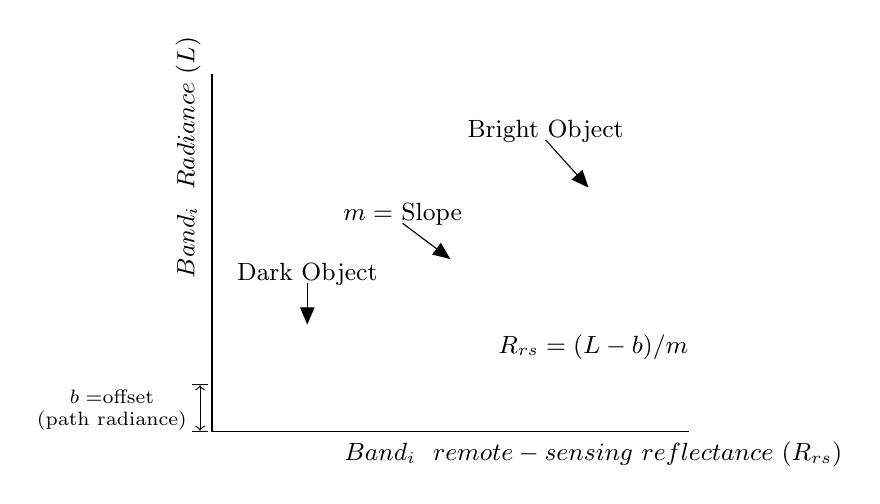
\begin{tikzpicture}[x=4ex,y=1ex]
 	%axis
	\draw (0,0) -- coordinate (x axis mid) (10,0);
    \draw (0,0) -- coordinate (y axis mid) (0,30);
 
    %labels      
	\node[below=0ex] at (8,0) {\small $Band_i~~remote-sensing~reflectance~(R_{rs})$};
	\node[rotate=90] at (-.5,23) {\small $Band_i~~Radiance~(L)$};

	\node[below=.2ex] at (-2.1,4.5) {\scriptsize $b=$offset};
	\node[below=1.4ex] at (-2.1,4.0) {\scriptsize (path radiance)};
	\draw[rotate=90,|<->|] (0,1) -- coordinate (x axis mid) (1,1);

	\node[below=0ex] at (2,15) {\small Dark Object};
	\draw[arrows=-triangle 45] (2,12.5) -- (2,9);

	\node[below=0ex] at (4,20) {\small $m=$ Slope};
	\draw[arrows=-triangle 45] (4,17.5) -- (5,14.5);

	\node[below=0ex] at (7,27) {\small Bright Object};
	\draw[arrows=-triangle 45] (7,24.5) -- (7.9,20.5);

	\node[below=0ex] at (8,9) {\small $R_{rs}=(L-b)/m$};

	%plots
	\draw plot 
		file {linereg.data};
	\draw plot[mark=*] 
		file {linereg2.data};

\end{tikzpicture}
% \caption{MoB-ELM atmospheric correction method. The MoB-ELM method is based on the traditional empirical line method (ELM). Two pixels from the image, the bright and dark pixel, are used to solve a liner regression with a slope $m$ and offset $b$ in the $R_{rs}$, $L$ space. Once this relationship is established, each $L$ value in the image can be converted to $R_{rs}$ through $R_{rs}=(L-b)/m$. \label{fig:ELMregression}
} % end resize
\end{figure}

     	\end{column}
\end{columns}

\vspace{.5cm}
\begin{itemize}
	\Large
	\item Two pixels in the scene with known reflectance: Bright and Dark pixels
	\vspace{0.3cm}
	% \item Linear relationship between radiance $L$ and reflectance $r_d$ 	
\end{itemize}
\end{frame}
% ----------------------------------- Slide ----------------------------------------------
\begin{frame}{\LARGE Our Approach:} 
{\Large Model-Based ELM (MoB-ELM)}

\begin{block}{\LARGE Bright Pixel}
 	\begin{itemize}
 	\Large
 		\item Radiance: PIF\footnotemark[1] from Landsat 8 image
 		\item Reflectance: PIF\footnotemark[1] from Landsat reflectance product
 	\end{itemize}
\end{block} 
% \vspace{0.1cm}
\begin{block}{\LARGE Dark Pixel}

	\begin{itemize}
	\Large
		\item Radiance: ROI\footnotemark[2] over water from Landsat 8 image
		\item Reflectance: Hydrolight
	\end{itemize}

\end{block}
\footnotetext[1]{Pseudo-Invariant Features}
\footnotetext[2]{Region of interest}

\end{frame}
% ----------------------------------- Slide ----------------------------------------------
\begin{frame}{\LARGE Model-Based ELM} 
{\vspace{.1cm} \Large Bright Pixel -- Pseudo-Invariant Features}

\begin{figure}[htb]
  \begin{minipage}[c]{0.48\linewidth}
    \centering
      \includegraphics[trim=30 0 30 0,clip,height=5cm]{/Users/javier/Desktop/Javier/PHD_RIT/Latex/Proposal/Images/DTROCL8falsecolor.jpg}  
    \vspace{0.3cm}
    \centerline{Downtown Rochester}
    \centerline{False Color Image}
  \end{minipage}
  \hfill
  \begin{minipage}[d]{0.48\linewidth}
    \centering
      \includegraphics[trim=30 0 30 0,clip,height=5cm]{/Users/javier/Desktop/Javier/PHD_RIT/Latex/Proposal/Images/PIFmaskApplied.jpg}
    \vspace{0.3cm}
    \centerline{Downtown Rochester}
    \centerline{PIF mask}
  \end{minipage}
  % \caption{PIF mask determination. (a) False color image, with vegetation in red and (b) PIF mask over downtown Rochester. \label{fig:PIFmask} } 
\end{figure}
\end{frame}

% % ----------------------------------- Slide ----------------------------------------------
% \begin{frame}{\LARGE Atmospheric Correction} 
% {\Large PIFs -- Bright Pixel}

% \begin{figure}[htb]
%   \begin{minipage}[c]{0.48\linewidth}
%     \centering
%       \includegraphics[height=4.8cm]{/Users/javier/Desktop/Javier/PHD_RIT/Latex/Proposal/Images/ZenithCorrection.eps}
%   % \caption{Mean values for nine scenes of the Landsat reflectance product after applying the master PIF mask. \label{fig:ZenithCorr} }   
%     \vspace{0.3cm}
%     \centerline{PIFs values for 9}
%     \centerline{Landsat reflectance images}
%   \end{minipage}
%   \hfill
%   \begin{minipage}[d]{0.48\linewidth}
%     \centering
%       \includegraphics[height=4.8cm]{/Users/javier/Desktop/Javier/PHD_RIT/Latex/Proposal/Images/ZenithCorrelation.eps}
%   % \caption{Linear regression between reflectance values and solar zenith angle for band 1 of the Landsat reflectance product. \label{fig:Band1Corr} }
%     \vspace{0.3cm}
%     \centerline{Band 1 - PIFs spectrum for 9}
%     \centerline{Landsat reflectance images}
%   \end{minipage}
%   % \caption{PIF mask determination. (a) False color image, with vegetation in red and (b) PIF mask over downtown Rochester. \label{fig:PIFmask} } 
% \end{figure}
% \end{frame}
% ----------------------------------- Slide ----------------------------------------------
\begin{frame}{\LARGE Model-Based ELM} 
{\vspace{.1cm} \Large Dark Pixel -- Hydrolight}

\begin{figure}[H]
		\includegraphics[height=6cm]{/Users/javier/Desktop/Javier/PHD_RIT/ConferencesAndApplications/2014_ASPRS_SOY/Images/HLdiagram.pdf}
\end{figure}
\hspace{5cm}{$*~$IOPs: Inherent Optical Properties}
\end{frame}
% ----------------------------------- Slide ----------------------------------------------
\begin{frame}{\LARGE Model-Based ELM} 
{\vspace{.1cm} \Large Dark Pixel -- Hydrolight}

\begin{columns}[c] % contents are top vertically aligned
  	\begin{column}[T]{6cm} % each column can also be its own environment

		\includegraphics[height=4cm]{/Users/javier/Desktop/Javier/PHD_RIT/ConferencesAndApplications/2014_RITResearchSymposium/Images/StudyArea.png}
	\end{column}

  	\begin{column}[T]{6cm} % each column can also be its own environment
  		\begin{itemize}
  			\item Radiance: Lake Ontario ROI
  			\vspace{.5cm}
  			\item Reflectance: Hydrolight with IOPs measured in the field over same ROI
  		\end{itemize}
 	\end{column}
\end{columns}

\end{frame}
% ----------------------------------- Slide ----------------------------------------------
\begin{frame}{\LARGE Model-Based ELM}{\vspace{.1cm} \Large Bright and Dark Pixel}

\begin{figure}[htb]
  \begin{minipage}[c]{0.48\linewidth}
    \centering
      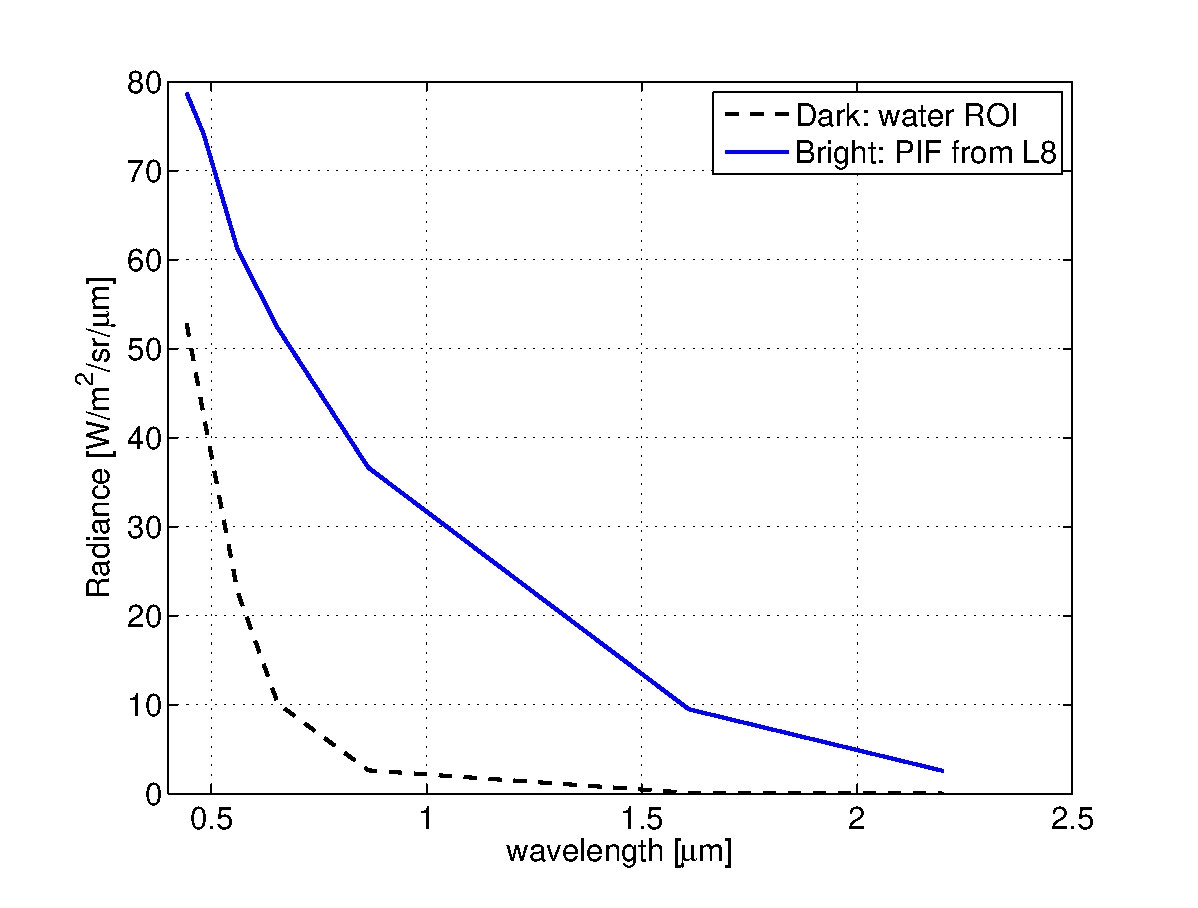
\includegraphics[width=6cm]{./Images/ELMrad130929_150422}
    \vspace{0.3cm}
    \centerline{(a) Radiance}\medskip
  \end{minipage}
  \hfill
  \begin{minipage}[d]{0.48\linewidth}
    \centering
      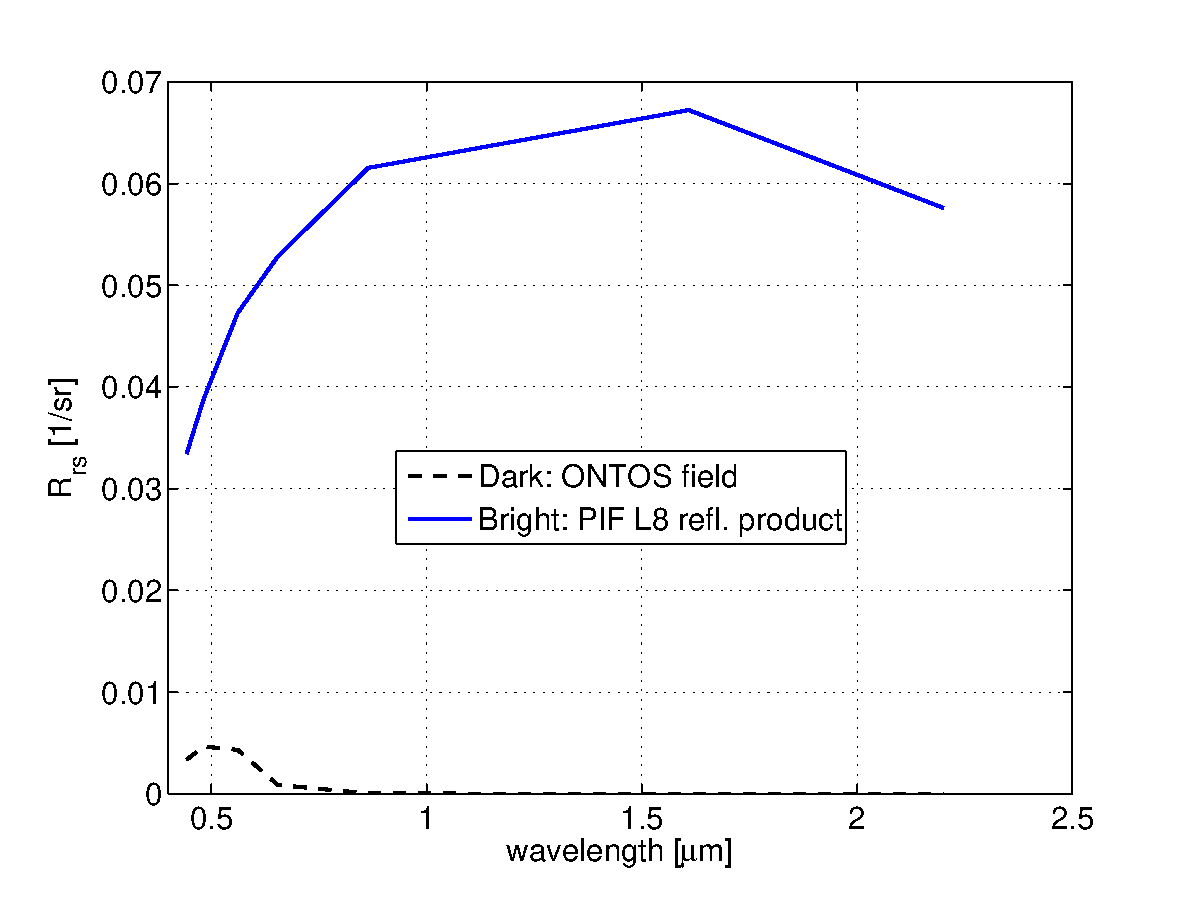
\includegraphics[width=6cm]{./Images/ELMRrs130929_150422}
    \vspace{0.3cm}
    \centerline{(b) $R_{rs}$}\medskip
  \end{minipage}
  % \caption{Example of the bright and dark pixel used in the MoB-ELM atmospheric correction method for Landsat 8 scene acquired on 09-19-2013.\label{fig:MOBELMpxls} } 
\end{figure}

\end{frame}
% ----------------------------------- Slide ----------------------------------------------
\begin{frame}{\LARGE Atmospheric Corrections Comparison}
\LARGE
\begin{itemize}\itemsep.5cm
	\item Our method (RIT): MoB-ELM
	\item Gordon and Wang's methods (NASA):
	\begin{itemize}
	\Large
		\item SeaDAS-SWIR
		\item SeaDAS-MUMM
		\item Acolite-SWIR
	\end{itemize}
\end{itemize}

\begin{block}{\large Gordon and Wang's tools}
\large
{\bf SEADAS:} NASA's Package for Ocean Color\\

{\bf ACOLITE:} Royal Belgian Institute of Natural Science
\end{block}

\end{frame}
% ----------------------------------- Slide ----------------------------------------------
\begin{frame}{\LARGE Atmospheric Corrections Comparison @ $443nm$}
\tiny
%^^^^^^^^^^^^^^^^^^^  FIGURE ^^^^^^^^^^^^^^^^^^^^^^^^^^^^^^^^^^^^^^^^^^^^
\begin{figure}[htbp!]
	\begin{minipage}[c]{0.48\linewidth}
  		\centering
  		\begin{overpic}[trim=0 200 0 0,clip,width=4.5cm]{./Images/subset_0_of_Collocated13262_ACOSWIR_MOB_SEA_Rrs_443MOBdivpi}
  		\put (5,5) {MOB-ELM}
  		\end{overpic}
  	\end{minipage}
  	\hfill
	\begin{minipage}[c]{0.48\linewidth}
  		\centering
  		\begin{overpic}[trim=0 200 0 0,clip,width=4.5cm]{./Images/subset_0_of_Collocated13262_ACOSWIR_MOB_SEA_Rrs_443ACO}
  		\put (5,5) {Acolite-SWIR}
  		\end{overpic}
  	\end{minipage}

	\begin{minipage}[c]{0.48\linewidth}
  		\centering
  		\begin{overpic}[trim=0 200 0 0,clip,width=4.5cm]{./Images/subset_0_of_Collocated13262_ACOSWIR_MOB_SEA_Rrs_443SEA}
  		\put (5,5) {SeaDAS-SWIR}
  		\end{overpic}
  	\end{minipage}
  	\hfill
	\begin{minipage}[c]{0.48\linewidth}
  		\centering
  		\begin{overpic}[trim=30 170 40 150,clip,width=4.5cm]{./Images/Collocated13262_ACOSWIR_MOB_SEA5x5_MUMM45_Rrs_443_MUMM45}
  		\put (5,5) {SeaDAS-MUMM}
  		\end{overpic}
  	\end{minipage}
  	\begin{minipage}[c]{1.0\linewidth}
  		\centering
  		\vspace{0.5cm}
  		\begin{overpic}[trim=0 0 0 0,clip,height=0.8cm]{./Images/Collocated13262_ACOSWIR_MOB_SEA5x5_MUMM45_colorbar}
  		\put (28,16) {$R_{rs}(443nm) [1/sr]$}
  		\end{overpic}
  	\end{minipage}

  % \caption{$R_{rs}$ 443.\label{fig:Rrs443} } 
\end{figure}

\end{frame}

% ----------------------------------- Slide ----------------------------------------------
\begin{frame}{\LARGE Atmospheric Corrections Comparison @ $561nm$}
\tiny
%^^^^^^^^^^^^^^^^^^^  FIGURE ^^^^^^^^^^^^^^^^^^^^^^^^^^^^^^^^^^^^^^^^^^^^
\begin{figure}[htbp!]
	\begin{minipage}[c]{0.48\linewidth}
  		\centering
  		\begin{overpic}[trim=0 155 40 150,clip,width=5cm]{./Images/Collocated13262_ACOSWIR_MOB_SEA5x5_MUMM45_Rrs_561_MOB}
  		\put (5,5) {MOB-ELM}
  		\end{overpic}
  	\end{minipage}
  	\hfill
	\begin{minipage}[c]{0.48\linewidth}
  		\centering
  		\begin{overpic}[trim=0 150 40 150,clip,width=5cm]{./Images/Collocated13262_ACOSWIR_MOB_SEA5x5_MUMM45_Rrs_561_ACO_R_R}
  		\put (5,5) {Acolite-SWIR}
  		\end{overpic}
  	\end{minipage}

	\begin{minipage}[c]{0.48\linewidth}
  		\centering
  		\begin{overpic}[trim=0 150 40 150,clip,width=5cm]{./Images/Collocated13262_ACOSWIR_MOB_SEA5x5_MUMM45_Rrs_561_SEA5x5_R}
  		\put (5,5) {SeaDAS-SWIR}
  		\end{overpic}
  	\end{minipage}
  	\hfill
	\begin{minipage}[c]{0.48\linewidth}
  		\centering
  		\begin{overpic}[trim=0 150 40 150,clip,width=5cm]{./Images/Collocated13262_ACOSWIR_MOB_SEA5x5_MUMM45_Rrs_561_MUMM45}
  		\put (5,5) {SeaDAS-MUMM}
  		\end{overpic}
  	\end{minipage}
  	

  	\begin{minipage}[c]{1.0\linewidth}
  		\centering
  		\vspace{0.3cm}
  		\begin{overpic}[trim=0 0 0 0,clip,height=0.8cm]{./Images/Collocated13262_ACOSWIR_MOB_SEA5x5_MUMM45_colorbar}
  		\put (28,16) {$R_{rs}(561nm) [1/sr]$}
  		\end{overpic}
  	\end{minipage}

  % \caption{$R_{rs}$ 561.\label{fig:Rrs561} } 
\end{figure}

\end{frame}

% ----------------------------------- Slide ----------------------------------------------
\begin{frame}{\LARGE Atmospheric Corrections Comparison @ $443nm$}%{\Large Methods Comparison }
% \tiny
\vspace{-.3cm}
%^^^^^^^^^^^^^^^^^^^  FIGURE ^^^^^^^^^^^^^^^^^^^^^^^^^^^^^^^^^^^^^^^^^^^^
\begin{figure}[htbp!]
  % \begin{minipage}[c]{0.49\linewidth}
  % 		\centering
  %     \begin{overpic}[trim=0 280 0 0,clip,width=4cm]{./Images/2013262_ACOMOBSEAMUM_443_Acolite-SWIR_SeaDAS-MUMM.png}
  %     % \put (65,17) {\large A) $443nm$}
  %     \end{overpic}  
  % \end{minipage}
  % \hfill
  \begin{minipage}[d]{0.49\linewidth}
  	\centering
      \begin{overpic}[trim=0 280 0 0,clip,width=4cm]{./Images/2013262_ACOMOBSEAMUM_443_Acolite-SWIR_MoB-ELM.png}
      % \put (65,17) {\large B) $483nm$}
      \end{overpic}
  \end{minipage}
  \hfill
  % \begin{minipage}[c]{0.49\linewidth}
  % 		\centering
  %     \begin{overpic}[trim=0 280 0 0,clip,width=4cm]{./Images/2013262_ACOMOBSEAMUM_443_Acolite-SWIR_SeaDAS-SWIR.png}
  %     % \put (65,17) {\large C) $561nm$}
  %     \end{overpic}  
  % \end{minipage}
  \begin{minipage}[d]{0.49\linewidth}
  	\centering
      \begin{overpic}[trim=0 280 0 0,clip,width=4cm]{./Images/2013262_ACOMOBSEAMUM_443_SeaDAS-MUMM_MoB-ELM.png}
      % \put (65,17) {\large D) $655nm$}
      \end{overpic}
  \end{minipage}
  % \hfill
  % \begin{minipage}[c]{0.49\linewidth}
  % 		\centering
  %     \begin{overpic}[trim=0 280 0 0,clip,width=4cm]{./Images/2013262_ACOMOBSEAMUM_443_SeaDAS-SWIR_SeaDAS-MUMM.png}
  %     % \put (65,17) {\large C) $561nm$}
  %     \end{overpic}  
  % \end{minipage}
  % \hfill
  \begin{minipage}[d]{0.49\linewidth}
  	\centering
      \begin{overpic}[trim=0 280 0 0,clip,width=4cm]{./Images/2013262_ACOMOBSEAMUM_443_SeaDAS-SWIR_MoB-ELM.png}
      % \put (65,17) {\large D) $655nm$}
      \end{overpic}
  \end{minipage}
  \hfill
  \begin{minipage}[d]{0.49\linewidth}
  	\centering
      \begin{overpic}[trim=70 00 0 1470,clip,width=4cm]{./Images/2013262_ACOMOBSEAMUM_655_Acolite-SWIR_SeaDAS-MUMM.png}
      \end{overpic}
  \end{minipage}    

% 
  % \caption{Scatter plots showing the comparison of remote-sensing reflectance ($R_{rs}$) at 443 nm, derived from the 09-29-2013 image over the Rochester Embayment (scene LC80160302013262LGN00) using the different methods. Colors denote pixel densities, the dashed black line is the 1:1 line, and the Reduced Major Axis (RMA) regression line is drawn in red. \label{fig:13262Rrs443} } 
\end{figure}

\end{frame}

% ----------------------------------- Slide ----------------------------------------------
\begin{frame}{\LARGE Atmospheric Corrections Comparison @ $561nm$}
\vspace{-.3cm}
%^^^^^^^^^^^^^^^^^^^  FIGURE ^^^^^^^^^^^^^^^^^^^^^^^^^^^^^^^^^^^^^^^^^^^^
\begin{figure}[htbp!]
  % \begin{minipage}[c]{0.49\linewidth}
  % 		\centering
  %     \begin{overpic}[trim=0 280 0 0,clip,width=4cm]{./Images/2013262_ACOMOBSEAMUM_561_Acolite-SWIR_SeaDAS-MUMM.png}
  %     % \put (65,17) {\large A) $443nm$}
  %     \end{overpic}  
  % \end{minipage}
  % \hfill
  \begin{minipage}[d]{0.49\linewidth}
  	\centering
      \begin{overpic}[trim=0 280 0 0,clip,width=4cm]{./Images/2013262_ACOMOBSEAMUM_561_Acolite-SWIR_MoB-ELM.png}
      % \put (65,17) {\large B) $483nm$}
      \end{overpic}
  \end{minipage}
  \hfill
  % \begin{minipage}[c]{0.49\linewidth}
  % 		\centering
  %     \begin{overpic}[trim=0 280 0 0,clip,width=4cm]{./Images/2013262_ACOMOBSEAMUM_561_Acolite-SWIR_SeaDAS-SWIR.png}
  %     % \put (65,17) {\large C) $561nm$}
  %     \end{overpic}  
  % \end{minipage}
  \begin{minipage}[d]{0.49\linewidth}
  	\centering
      \begin{overpic}[trim=0 280 0 0,clip,width=4cm]{./Images/2013262_ACOMOBSEAMUM_561_SeaDAS-MUMM_MoB-ELM.png}
      % \put (65,17) {\large D) $655nm$}
      \end{overpic}
  \end{minipage}
  % \hfill
  % \begin{minipage}[c]{0.49\linewidth}
  % 		\centering
  %     \begin{overpic}[trim=0 280 0 0,clip,width=4cm]{./Images/2013262_ACOMOBSEAMUM_561_SeaDAS-SWIR_SeaDAS-MUMM.png}
  %     % \put (65,17) {\large C) $561nm$}
  %     \end{overpic}  
  % \end{minipage}
  % \hfill

  \begin{minipage}[d]{0.49\linewidth}
  	\centering
      \begin{overpic}[trim=0 280 0 0,clip,width=4cm]{./Images/2013262_ACOMOBSEAMUM_561_SeaDAS-SWIR_MoB-ELM.png}
      % \put (65,17) {\large D) $655nm$}
      \end{overpic}
  \end{minipage}
  \hfill
  \begin{minipage}[d]{0.49\linewidth}
  	\centering
      \begin{overpic}[trim=70 0 0 1470,clip,width=4cm]{./Images/2013262_ACOMOBSEAMUM_655_Acolite-SWIR_SeaDAS-MUMM.png}
      \end{overpic}
  \end{minipage}    

% 
  % \caption{Scatter plots showing the comparison of remote-sensing reflectance ($R_{rs}$) at 561 nm, derived from the 09-29-2013 image over the Rochester Embayment (scene LC80160302013262LGN00) using the the different methods. Colors denote pixel densities, the dashed black line is the 1:1 line, and the Reduced Major Axis (RMA) regression line is drawn in red. \label{fig:13262Rrs655} } 
\end{figure}


\end{frame}


% ----------------------------------- Slide ----------------------------------------------
\begin{frame}{\LARGE Atmospheric Correction Methods} 
{\Large Comparison with Field Data}
% \centerline{\LARGE Bright and Dark Pixel}
\tiny
%^^^^^^^^^^^^^^^^^^^  FIGURE ^^^^^^^^^^^^^^^^^^^^^^^^^^^^^^^^^^^^^^^^^^^^
\begin{figure}[htbp!]
  \begin{minipage}[c]{0.325\linewidth}
  		\centering
      \begin{overpic}[trim=0 0 0 0,clip,width=3.7cm]{./Images/RrsCompONTNS.png}
      \put (20,60) {A) ONTNS} 
      \end{overpic}  
  \end{minipage}
  \hfill
  \begin{minipage}[d]{0.325\linewidth}
  	\centering
      \begin{overpic}[trim=0 0 0 0,clip,width=3.7cm]{./Images/RrsCompONTOS.png}
      \put (20,14) {B) ONTOS}  	 	
      \end{overpic}
  \end{minipage}
  \hfill
  \begin{minipage}[d]{0.325\linewidth}
  	\centering
      \begin{overpic}[trim=0 0 0 0,clip,width=3.7cm]{./Images/RrsCompONTEX.png}
      \put (20,14) {C) ONTEX}  	
      \end{overpic}
  \end{minipage}

  \begin{minipage}[c]{0.49\linewidth}
  		\centering
      \begin{overpic}[trim=0 0 0 0,clip,width=3.7cm]{./Images/RrsCompRVRPL.png}
      \put (20,14) {D) RVRPLM}  		
      \end{overpic}  
  \end{minipage}
  \hfill
  \begin{minipage}[c]{0.49\linewidth}
  		\centering
      \begin{overpic}[trim=0 0 0 0,clip,width=3.7cm]{./Images/RrsCompRVRPI.png}
      \put (20,14) {E) RVRPIER}  		
      \end{overpic}  
  \end{minipage}
  
  % \caption{Comparison of $R_{rs}$ for the sites on the 90-19-2013 collection. \label{fig:13262RrsComp}} 
\end{figure}

\end{frame}
% ----------------------------------- Slide ----------------------------------------------
\begin{frame}{\LARGE Atmospheric Correction Methods} 
{\Large Comparison with Field Data}
% \centerline{\LARGE Bright and Dark Pixel}

\begin{block}{$R_{rs}(\lambda)$ normalized root mean squared error (NRMSE)}
	\begin{equation*}
\label{eq:NRMSE}
	NRMSE =\frac{\sqrt{\frac{1}{N}\sum_{n=1}^N{\left[R_{rs}(\lambda)_{ret}(n) - R_{rs}(\lambda)_{mea}(n)\right]^2}}}{max\{R_{rs}(\lambda)_{mea}(n)\} - min\{R_{rs}(\lambda)_{mea}(n)\}}\times100 ~[\%]
\end{equation*}
\end{block}

\noindent where:\\
		$R_{rs}(\lambda)_{ret}$: retrieved\\
	 	$R_{rs}(\lambda)_{mea}$: measured $R_{rs}(\lambda)$\\
	 	$n=1\dots N$: number of samples.

\end{frame}
% ----------------------------------- Slide ----------------------------------------------
\begin{frame}{\LARGE Atmospheric Correction Methods} 
{\Large Comparison with Field Data}
% \centerline{\LARGE Bright and Dark Pixel}
\tiny
%^^^^^^^^^^^^^^^^^^^  FIGURE ^^^^^^^^^^^^^^^^^^^^^^^^^^^^^^^^^^^^^^^^^^^^
\begin{figure}[htbp!]
  \begin{minipage}[c]{0.48\linewidth}
  		\centering
      \begin{overpic}[trim=110 0 140 0,clip,width=5.5cm]{./Images/NRMSE_RRS_B1.png}
      \put (20,40) {A) 443nm} 
      \end{overpic}  
  \end{minipage}
  \hfill
  \begin{minipage}[d]{0.48\linewidth}
  	\centering
      \begin{overpic}[trim=110 0 140 0,clip,width=5.5cm]{./Images/NRMSE_RRS_B2.png}
      \put (20,40) {B) 483nm}  	 	
      \end{overpic}
  \end{minipage}

    \begin{minipage}[c]{0.48\linewidth}
  		\centering
      \begin{overpic}[trim=110 0 140 0,clip,width=5.5cm]{./Images/NRMSE_RRS_B3.png}
      \put (20,40) {A) 561nm} 
      \end{overpic}  
  \end{minipage}
  \hfill
  \begin{minipage}[d]{0.48\linewidth}
  	\centering
      \begin{overpic}[trim=110 0 140 0,clip,width=5.5cm]{./Images/NRMSE_RRS_B4.png}
      \put (20,40) {B) 655nm}  	 	
      \end{overpic}
  \end{minipage}

  % \caption{NRMSE for $R_{rs}$ at 443, 483, 561 and 655nm.\label{fig:NRMSE130919_RRS} } 
\end{figure}

\end{frame}
%%%%%%%%%%%%%%%%%%%%%%%%%%%%%%%%%%%%%%%%%%%%%%%%%%%%%%%%%%%%%%%%%%%%%%%%%%%%%%%%%%%%%%%%%%
\section[Chl-{\it a} Retrieval]{Chlorophyll-{\it a} Retrieval}
\subsection*{}
% ----------------------------------- Slide ----------------------------------------------
\begin{frame}{\LARGE Chlorophyll-{\it a} Retrieval Process} 

\begin{figure}[H]
		\includegraphics[height=7cm]{/Users/javier/Desktop/Javier/PHD_RIT/ConferencesAndApplications/2014_ASPRS_SOY/Images/RetProcess.pdf}
\end{figure}

\end{frame}
% ----------------------------------- Slide ----------------------------------------------

\begin{frame}{\LARGE Chl-{\it a} Retrieval}{\vspace{0.1cm} \large RIT's Spectral Matching and LUT Algorithm}
% \begin{block}{\footnotesize LUT}
  \begin{columns}[c] % contents are top vertically aligned
  	\begin{column}[T]{6cm} % each column can also be its own environment
  	\vspace{0.2cm}
    	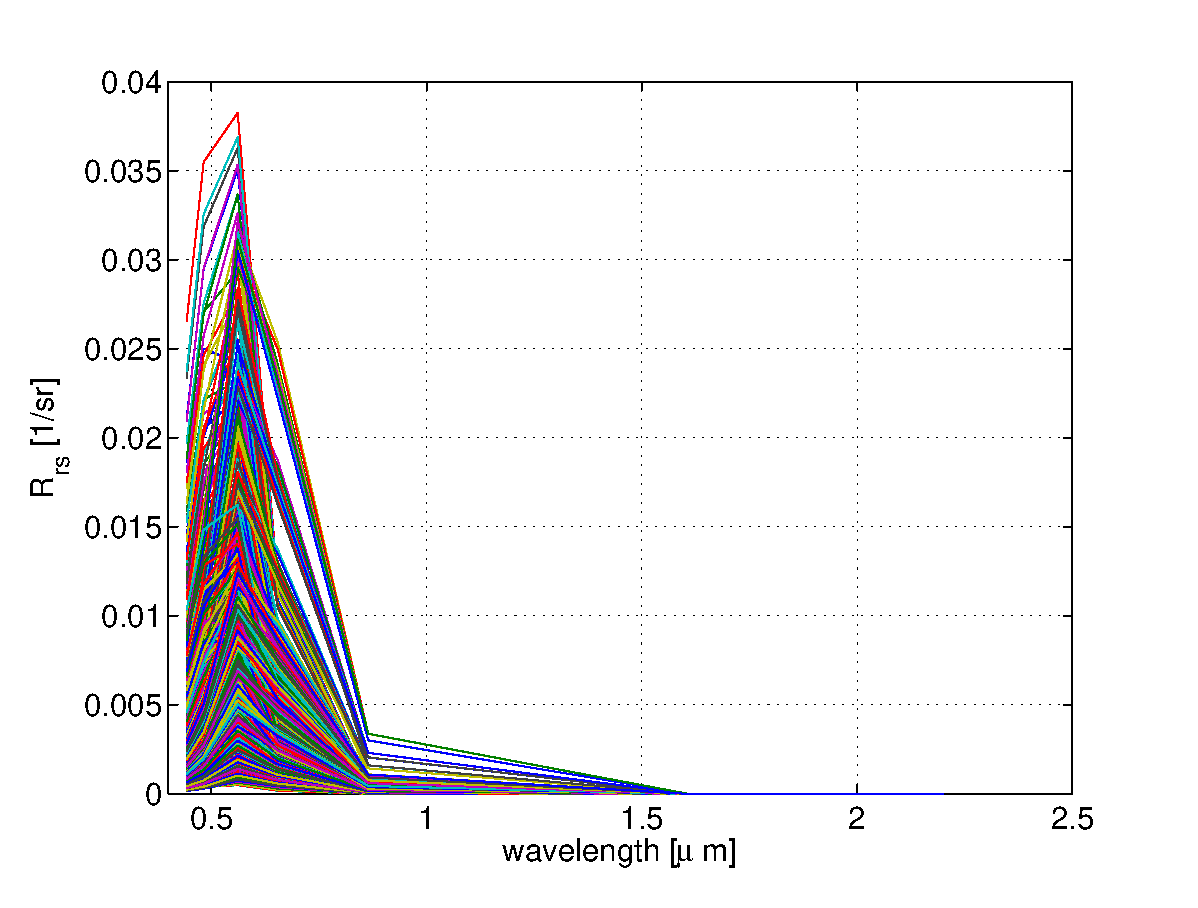
\includegraphics[height=5cm]{/Users/javier/Desktop/Javier/PHD_RIT/ConferencesAndApplications/2015_Landsat_Special_Issue/Images/LUTsmart130919_150422.eps}
    	    \vspace{0.2cm}
    		\centerline{LUT from Hydrolight}
    		\centerline{(Known concentrations)}
    \end{column}
  	\hspace{.3cm}
  	\begin{column}[T]{6cm} % each column can also be its own environment
  	\vspace{0.2cm}
	\scriptsize \addtolength{\tabcolsep}{-5pt}
\begin{table}[htb]
% \caption{Input parameters for the LUT generation in Hydrolight for the Landsat 8 image acquired on 09-19-2013. \label{tab:LUTconc}} 
\tiny
\centering
    \begin{tabular}{ccccc}
    \hline \hline
            IOPs Input & \bfseries{$C_a$} & \bfseries{$TSS$} & \bfseries{$a_{CDOM}(440nm)$} & \bfseries{$b_b/b$}    \\
                   & $[mg~m^{-3}]$        & $[g~m^{-3}]$       &  $[1/m]$           & $[\%]$            \\ \hline \hline
\multirow{8}{*}{ONTNS}  &  0.1    	& 1.0     &  0.11   &  0.3  \\
   	&  0.5    	& 2.0   &  0.15   	&  0.4  \\
    &  1.0    	& 5.0   &  0.21   	&  0.5  \\
    &  3.0    	& 10.0  &  0.6    	&  0.6  \\ 
    &  10.0     & --    &  --   	&  0.7  \\  
    &  20.0     & --    &  --   	&  1.0  \\  
    &  40.0     & --    &  --   	&  1.4  \\
    &  --       & --    &  --   	&  2.0  \\ \hline

\multirow{8}{*}{LONGS}   &  60.0   & 25.0    &  1.0    &  0.3  \\
    &  90.0   & 45.0    &  1.2    &  0.4  \\
    &  110.0  & 50.0    &  --     &  0.5  \\
    &  --     & --      &  --     &  0.6  \\  
    &  --     & --      &  --     &  0.7  \\  
    &  --     & --      &  --     &  1.0  \\   
    &  --     & --      &  --     &  1.4  \\  
    &  --     & --      &  --     &  2.0  \\  \hline \hline
% --      &  135.0  & --      &  --     &  --   \\  
% --      &  150.0  & --      &  --     &  --   \\ \hline 
    \end{tabular}
  \end{table}
     	\end{column}
\end{columns}
% \end{block}
\end{frame}

% ----------------------------------- Slide ----------------------------------------------
\begin{frame}{\LARGE Chl-{\it a} Retrieval}{\vspace{0.1cm} \Large NASA's OC3 Algorithm}


% \begin{block}{\footnotesize LUT}
\begin{columns}[c] % contents are top vertically aligned
  	\begin{column}[T]{5cm} % each column can also be its own environment
  	\vspace{0.4cm}
    	\includegraphics[height=5cm]{./Images/OC4_OReilly.png}\\
    	*\cite{OReilly2000}
    \end{column}
  	% \hspace{.3cm}
  	\begin{column}[T]{6.5cm} % each column can also be its own environment
  	\vspace{1cm}
	% \scriptsize \addtolength{\tabcolsep}{-5pt}
		\begin{equation*}
			\begin{gathered}
			C_a = 10^{\gamma}\\
			\gamma = a_0+a_1\chi+a_2\chi^2+a_3\chi^3+a_4\chi^4\\
			\chi = log_{10}(R)\\
			R = \frac{max(R_{rs}(443,483))}{R_{rs}(561)}
			\end{gathered}
		\end{equation*}
    \end{column}
\end{columns}
% \end{block}

\end{frame}

% ----------------------------------- Slide ----------------------------------------------
\begin{frame}{\LARGE Chl-{\it a} Retrieval}{\vspace{.1cm} \Large Methods Comparison}

%^^^^^^^^^^^^^^^^^^^  FIGURE ^^^^^^^^^^^^^^^^^^^^^^^^^^^^^^^^^^^^^^^^^^^^
\begin{figure}[htbp!]
	\begin{minipage}[c]{0.48\linewidth}
  		\centering
  		\begin{overpic}[trim=0 0 40 0,clip,width=5cm]{./Images/Collocated13262_ACOSWIR_MOB_SEA5x5_MUMM45_chlor_MOB_D_R_R}
  		\put (5,5) {MOB-ELM}
  		\end{overpic}
  	\end{minipage}
  	\hfill
	\begin{minipage}[c]{0.48\linewidth}
  		\centering
  		\begin{overpic}[trim=0 0 40 0,clip,width=5cm]{./Images/LC80160302013262LGN00_L2_SWIR_FranzAve_chlor_a_ACO_OC3def}
  		\put (5,5) {Acolite-SWIR}
  		\end{overpic}
  	\end{minipage}

	\begin{minipage}[c]{0.48\linewidth}
  		\centering
  		\begin{overpic}[trim=0 0 40 0,clip,width=5cm]{./Images/Collocated13262_ACOSWIR_MOB_SEA5x5_MUMM45_chlor_a_SEA5x5_R}
  		\put (5,5) {SeaDAS-SWIR}
  		\end{overpic}
  	\end{minipage}
  	\hfill
	\begin{minipage}[c]{0.48\linewidth}
  		\centering
  		\begin{overpic}[trim=0 0 40 0,clip,width=5cm]{./Images/Collocated13262_ACOSWIR_MOB_SEA5x5_MUMM45_chlor_a_MUMM45}
  		\put (5,5) {SeaDAS-MUMM}
  		\end{overpic}
  	\end{minipage}
  	

  	\begin{minipage}[c]{1.0\linewidth}
  		\centering
  		\vspace{0.5cm}
  		\begin{overpic}[trim=0 0 0 0,clip,height=1.2cm]{./Images/Collocated13262_ACOSWIR_MOB_SEA5x5_MUMM45_colorbar_CHL_0_100}
  		\put (35,16) {$C_a [mg/m^3]$}
  		\end{overpic}
  	\end{minipage}

  % \caption{$C_a.$ \label{fig:chlor_a} } 
\end{figure}

\end{frame}
% ----------------------------------- Slide ----------------------------------------------
\begin{frame}{\LARGE Chl-{\it a} Retrieval}{\vspace{.1cm} \Large Comparison with Field Data}
%^^^^^^^^^^^^^^^^^^^  FIGURE ^^^^^^^^^^^^^^^^^^^^^^^^^^^^^^^^^^^^^^^^^^^^
\begin{figure}[htbp!]
  \begin{minipage}[c]{1.0\linewidth}
		\centering
     	\begin{overpic}[trim=0 0 0 0,clip,width=7cm]{./Images/CHLmeavsret.png}
    	% \put(17,62){\includegraphics[trim=10 80 0 0,clip,width=2.5cm]{./Images/CHLmeavsretZOOM.png}}
      \end{overpic}  
  \end{minipage}
  % \caption{Comparison retrieved versus measured $R_{rs}$ for the sites on the 90-19-2013 collection. \label{fig:13262RrsMeaVSRet}} 
\end{figure}
\end{frame}

% ----------------------------------- Slide ----------------------------------------------
\begin{frame}{\LARGE Chl-{\it a} Retrieval}{\vspace{.1cm} \Large Comparison with Field Data}

\begin{block}{$C_a$ normalized root mean squared error (NRMSE)}

\begin{equation*}
\label{eq:NRMSEchl}
	NRMSE =\frac{\sqrt{\frac{1}{N}\sum_{n=1}^N{\left[C_{ret}(n) - C_{mea}(n)\right]^2}}}{max\{C_{mea}(n)\} - min\{C_{mea}(n)\}}\times100 ~[\%]
\end{equation*}
\end{block}

\noindent where:\\
$C_{ret}$: retrieved concentration\\
$C_{mea}$: measured concentration\\
$n=1\dots N$: number of samples.

\end{frame}


% ----------------------------------- Slide ----------------------------------------------
\begin{frame}{\LARGE Chl-{\it a} Retrieval}{\vspace{.1cm} \Large Comparison with Field Data}

%^^^^^^^^^^^^^^^^^^^  FIGURE ^^^^^^^^^^^^^^^^^^^^^^^^^^^^^^^^^^^^^^^^^^^^
\begin{figure}[htbp!]
  \centering
  \includegraphics[height=7.0cm]{./Images/13262_NRMSE_CHL.png}
  % \caption{NRMSE for $C_a$.\label{fig:NRMSE130919} } 
\end{figure}

\end{frame}
%%%%%%%%%%%%%%%%%%%%%%%%%%%%%%%%%%%%%%%%%%%%%%%%%%%%%%%%%%%%%%%%%%%%%%%%%%%%%%%%%%%%%%%%%%
\section{Summary and Conclusions}
\subsection*{Conclusions}
% ----------------------------------- Slide ----------------------------------------------
\begin{frame}{\LARGE Summary}
\Large
\begin{itemize}\itemsep.5cm
\setbeamercovered{transparent}
    \uncover<2->{
	\item Two kind of atmospheric algorithms were tested: MoB-ELM (RIT) and Gordon and Wang's (NASA)}
	\uncover<3->{
	\item MoB-ELM: Based on ELM with Bright and Dark pixel from models }
	\uncover<4->{
	\item The retrieval of Chlorophyll-{\it a} was applied for both outcomes}
\end{itemize}


\end{frame}
% ----------------------------------- Slide ----------------------------------------------
\begin{frame}{\LARGE Conclusions} 
\begin{itemize}
\Large
\setbeamercovered{transparent}
    \uncover<2->{
	\item Landsat 8 has a great potential to help in fresh and coastal water quality studies}
	\vspace{\baselineskip}
	\uncover<3->{
	\item Standard Atmospheric Correction algorithms do not work in highly turbid waters}
	\vspace{\baselineskip}
	\uncover<4->{
	\item MoB-ELM is a potential solution. It can be applied to many cases, but not all of them}
\end{itemize}
\end{frame}
 % ----------------------------------- Slide ----------------------------------------------
% \section*{}
% \begin{frame}%[shrink=30] 
% \tiny
%   \frametitle{References}
%   \nocite{*}
%   \bibliographystyle{apalike}
%   \bibliography{HLbeamerbib}
% \end{frame}

%% ----------------------------------- Slide ----------------------------------------------

{	
\setbeamertemplate{footline}{} 
\setbeamertemplate{headline}{}
\begin{frame}[noframenumbering] 

% \vspace{\baselineskip}
% \centerline{\Large Thanks for your attention!}
	% \vspace{\baselineskip}

% \centerline{\Huge QUESTIONS?}
\uncover <2->{\centerline{\Huge QUESTIONS?}}
\vspace{\baselineskip}
\centerline{Javier A. Concha}
\centerline{jxc4005@rit.edu}

\begin{figure}[htb]
\centering
\includegraphics[height=6cm]{./Images/AlgaBloom}
\end{figure}
\vspace{-.3cm}
{\hspace{0.3cm} \tiny $*~$Western Lake Erie Basin's developing algal bloom, on July 28, 2015. Credit: NASA Earth Observatory}
\end{frame}
}
% #################################################################################
% ########################## END PRESENTATION #####################################
% #################################################################################
\appendix
\section{Additional Material}
% ----------------------------------- Slide ----------------------------------------------
% ------------------------------ SUBSECTION ----------------------------------------------
\subsection*{Field Collection and Lab Measurements}
\begin{frame}{\LARGE Field Collection} 
\begin{figure}[htb]
  \centering
  \includegraphics[width=8cm]{/Users/javier/Desktop/Javier/PHD_RIT/Latex/Proposal/Images/groundtruth-sitenames-no-ends.jpg}
  % \caption{Sites in the Rochester Embayment for the water sample collection on September, $19^{th}$, 2013.\label{fig:0910913Sites} } 
\end{figure}
\end{frame}
% ----------------------------------- Slide ----------------------------------------------
\begin{frame}{\LARGE Field Collection (con't)} 
\vspace{-1cm}
\begin{figure}[htb]
\centering
\includegraphics[height=7cm]{/Users/javier/Desktop/Javier/PHD_RIT/ConferencesAndApplications/2014_ASPRS_SOY/Images/Collection.pdf}
      
\end{figure}
% \centerline{Comparison between traditional ELM (dashed lines)}
% \centerline{and model-based ELM (solid lines).}
\end{frame}
% ----------------------------------- Slide ----------------------------------------------
\begin{frame}{\LARGE Lab Measurements} 
\vspace{-1cm}
\begin{figure}[htb]
\centering
\includegraphics[height=7cm]{/Users/javier/Desktop/Javier/PHD_RIT/ConferencesAndApplications/2014_ASPRS_SOY/Images/LabMeasurements.pdf}
      
\end{figure}
% \centerline{Comparison between traditional ELM (dashed lines)}
% \centerline{and model-based ELM (solid lines).}
\end{frame}

% --- slide ------------------------------------------------
\begin{frame}{\LARGE Atmospheric Correction}{\Large \cite{Gordon:1994} Methods}
\begin{itemize}
\Large
\item Atmospheric correction used for Ocean Color Satellites (i.e. CZCS, MODIS, SeaWiFS) are based on the work done by \cite{Gordon:1994}: ``Retrieval of water-leaving radiance and aerosol optical thickness over the oceans with SeaWiFS: a preliminary algorithm.''

\end{itemize}
\end{frame}
% --- slide ------------------------------------------------
\begin{frame}{\LARGE Atmospheric Correction}{\Large \cite{Gordon:1994} Methods (con't)}

\Large
\begin{block}{Apparent reflectance, \LARGE $\rho$}
\begin{equation}\label{eq:rho}
  \rho = \frac{\pi L}{F_o \cos{\theta}}\notag
\end{equation}
\end{block}
where:\\
\begin{itemize}\itemsep.2cm
\item{ $L$: upward radiance in the given viewing direction}\\
\item{ $F_o$: exoatmospheric irradiance}\\
\item{ $\theta$: solar-zenith angle}
\end{itemize}
\end{frame}
% --- slide ------------------------------------------------
\begin{frame}{\LARGE Atmospheric Correction}{\Large \cite{Gordon:1994} Methods (con't)}

\begin{block}{Reflectance at the TOA, $\rho_t$}
\begin{equation}\label{eq:rho_t}
  \rho_t(\lambda) = \rho_r(\lambda) + \rho_a(\lambda) + \rho_{ra}(\lambda) + T_v[\rho_w(\lambda) + \rho_{wc}(\lambda)]\notag
\end{equation}
\end{block}

\begin{itemize}\itemsep.2cm
\item {$\rho_r(\lambda)$: reflectance due to multiple scatter by air molecules only (Rayleigh scattering)}\\

\item {$\rho_a(\lambda)$: reflectance due to multiple scatter by aerosols only}\\

\item {$\rho_{ra}(\lambda)$: reflectance due to the interaction between Rayleigh and aerosol scattering}\\

\item {$T_v(\lambda)$: diffuse atmospheric transmittance from the water to the sensor}\\

\item {$\rho_{wc}(\lambda)$: glint}\\

\item {$\rho_w(\lambda)$: water-leaving reflectance}

\end{itemize}

\end{frame}

% --- slide ------------------------------------------------
\begin{frame}{\LARGE Atmospheric Correction}{\Large \cite{Gordon:1994} Methods (con't)}
\Large
\begin{block}{Reflectance at the TOA, $\rho_t$}
\begin{equation}\label{eq:rho_t}
  \rho_t(\lambda) = \rho_r(\lambda) + \rho_a(\lambda) + \rho_{ra}(\lambda) + T_v[\rho_w(\lambda) + \rho_{wc}(\lambda)]\notag
\end{equation}
\end{block}
\vspace{.3cm}
\begin{itemize}\itemsep.2cm
	\item{ \cite{Gordon:1994} estimate $\rho_a(\lambda) + \rho_{ra}(\lambda)$ in the visible (VIS) using an estimation of $\rho_a(\lambda) + \rho_{ra}(\lambda)$ in the near infrared (NIR).}
\end{itemize}

\end{frame}
% --- slide ------------------------------------------------
\begin{frame}{\LARGE Atmospheric Correction}{\Large \cite{Gordon:1994} Methods (con't)}
\Large
\begin{block}{Rayleigh and glint corrected, $\rho_c$}
	\begin{equation}
		 \rho_c(\lambda) = \rho_a(\lambda) + \rho_{ra}(\lambda) + T_v(\lambda)\rho_{w}(\lambda)\notag
	\end{equation}
\end{block}	

\begin{block}{Single Scattering Approximation}
\begin{equation}\label{eq:singleapprox}
  \rho_a(\lambda)+\cancel{\rho_{ra}(\lambda)} \approx \rho_{as}(\lambda)\notag
\end{equation}
\end{block}	

\begin{block}{Black Pixel Assumption}
	\begin{equation}
		 \rho_w(\lambda_{NIR}) \approx 0 \Rightarrow \rho_c(\lambda_{NIR}) = \rho_{as}(\lambda_{NIR})\notag
	\end{equation}
\end{block}
\end{frame}
% --- slide ------------------------------------------------
\begin{frame}{\LARGE Atmospheric Correction}{\Large \cite{Gordon:1994} Methods (con't)}
\large

\begin{block}{Single Scattering Epsilon (SSE) \cite{Gordon:1994}}
\begin{equation}
  \varepsilon(\lambda_{NIR1},\lambda_{NIR2}) \equiv \frac{\rho_{as}(\lambda_{NIR1})}{\rho_{as}(\lambda_{NIR2})}\notag
\end{equation}
\end{block}


\begin{block}{For the VIS}
\begin{equation}\label{eq:rholambda_i}
  \rho_{as}(\lambda_{VIS}) = \varepsilon(\lambda_{VIS},\lambda_{NIR2})\rho_{as}(\lambda_{NIR2})\notag
\end{equation}
\end{block}


\end{frame}
% --- slide ------------------------------------------------
\begin{frame}{\LARGE Atmospheric Correction}{\Large \cite{Gordon:1994} Methods (con't)}

\begin{figure}[htb]
  \centering
  \includegraphics[width=8cm,clip=true]{/Users/javier/Desktop/Javier/PHD_RIT/Latex/Proposal/Images/epsilonvslambdaGordon.png}
  \caption{$\varepsilon(\lambda,\lambda_{NIR2})$ values in natural logaritmic scale for different aerosol models and relative humidity (Source: \cite{Gordon:1997}). \label{fig:epsilonvslambda} } 
  % \vspace{0.5cm}
\end{figure}

\end{frame}
% --- slide ------------------------------------------------
\begin{frame}{\LARGE Atmospheric Correction}{\Large \cite{Gordon:1994} Methods (con't)}

\begin{figure}[htb]
  \centering
  \includegraphics[width=5cm,clip=true]{/Users/javier/Desktop/Javier/PHD_RIT/Latex/Proposal/Images/epsilonvslambdaGordon.png} 
  \vspace{-0.7cm}
\end{figure}

% \begin{block}{For several aerosols}
\begin{gather*}\label{eq:epsilonexp}
  \varepsilon(\lambda_{VIS},\lambda_{NIR2}) = \frac{\rho_{as}(\lambda_{VIS})}{\rho_{as}(\lambda_{NIR2})} \approx exp[c(\lambda_{VIS}-\lambda_{NIR2})]\notag \\
  \Rightarrow \rho_{as}(\lambda_{VIS}) = exp[c(\lambda_{VIS}-\lambda_{NIR2})]\rho_{as}(\lambda_{NIR2})
  \notag
\end{gather*}
\vspace{-0.3cm}
where:\\
\begin{equation}
  \varepsilon(\lambda_{NIR1},\lambda_{NIR2}) = \frac{\rho_{as}(\lambda_{NIR1})}{\rho_{as}(\lambda_{NIR2})} \approx exp[c(\lambda_{NIR1}-\lambda_{NIR2})]\Rightarrow c \notag
\end{equation}
% \end{block}

\end{frame}

% --- slide ------------------------------------------------
\section*{}
\begin{frame}%[shrink=30] 
\tiny
  \frametitle{References}
  % \nocite{*}
  \bibliographystyle{apalike}
  \bibliography{/Users/javier/Desktop/Javier/PHD_RIT/Latex/javier_bib}
\end{frame}
% ----------------------------------- Slide ----------------------------------------------
\begin{frame}{\LARGE Atmospheric Correction}{\Large Methods Comparison}
% \centerline{\LARGE Bright and Dark Pixel}

\begin{table}[!ht]
% \caption{ Comparison different methods for retrieving $R_{rs}$. \label{tab:RrsCompMethod} } 
\centering
\tiny
\begin{tabular}{cllcccccccc} 
 % \bfseries{Band n} & \bfseries{$m$}      & \bfseries{$y_0$}    & \bfseries{$R^2$}     & \bfseries{$RMSE$} & $y(x=45^\circ)$   \\ \hline \hline
Band		&   Method 1      &  Method 2	  &	Slope  	&	Offset  &	$R^2 $  &	N      	&	RMSE    	\\ 
$[nm]$		&	  		      &  		 	  &	  		&			&	   		&	     	&$[mg/m^3]$ 	\\	\hline \hline
\multirow{6}{*}{443}&Acolite-SWIR&MoB-ELM     &	0.9444 	&	-0.0047 &	0.8791 	&	144047  &	0.0054  	\\
			&   SeaDAS-SWIR   &  MoB-ELM      &	0.8664 	&	-0.0007 &	0.7637 	&	141563  &	0.0019  	\\
			&   SeaDAS-MUMM   &  MoB-ELM      &	0.8811 	&	-0.0018 &	0.7474 	&	144947  &	0.0029  	\\
			&   Acolite-SWIR  &  SeaDAS-SWIR  &	1.1437 	&	-0.0053 &	0.7804 	&	145186  &	0.0038  	\\
			&   Acolite-SWIR  &  SeaDAS-MUMM  &	1.0600 	&	-0.0032 &	0.8554 	&	147730  &	0.0026  	\\
			&   SeaDAS-SWIR   &  SeaDAS-MUMM  &	0.9175 	&	~0.0018 &	0.8456 	&	145315  &	0.0014  	\\  \hline
\multirow{6}{*}{448}&Acolite-SWIR&MoB-ELM     &	0.9353 	&	-0.0030 &	0.9302 	&	144077  &	0.0037  	\\
			&   SeaDAS-SWIR   &  MoB-ELM      &	0.8547 	&	~0.0002 &	0.8454 	&	142116  &	0.0014  	\\
			&   SeaDAS-MUMM   &  MoB-ELM      &	0.8639 	&	-0.0007 &	0.8408 	&	145138  &	0.0022  	\\ 
			&   Acolite-SWIR  &  SeaDAS-SWIR  &	1.1269 	&	-0.0041 &	0.8739 	&	145692  &	0.0028  	\\
			&   Acolite-SWIR  &  SeaDAS-MUMM  &	1.0693 	&	-0.0024 &	0.9175 	&	147837  &	0.0018  	\\
			&   SeaDAS-SWIR   &  SeaDAS-MUMM  &	0.9441 	&	~0.0015 &	0.9122 	&	145888  &	0.0012  	\\ \hline
\multirow{6}{*}{561}&Acolite-SWIR&  MoB-ELM   &	1.0183 	&	-0.0011 &	0.9044 	&	144192  &	0.0011  	\\
	 		&   SeaDAS-SWIR   &  MoB-ELM      &	1.0043 	&	~0.0001 &	0.7828 	&	143288  &	0.0009  	\\
	 		&   SeaDAS-MUMM   &  MoB-ELM      &	1.0611 	&	-0.0010 &	0.8468 	&	145339  &	0.0009  	\\
	 		&   Acolite-SWIR  &  SeaDAS-SWIR  &	1.0307 	&	-0.0013 &	0.8233 	&	146761  &	0.0013  	\\
	 		&   Acolite-SWIR  &  SeaDAS-MUMM  &	0.9663 	&	-0.0001 &	0.8968 	&	148040  &	0.0007  	\\
	  		&   SeaDAS-SWIR   &  SeaDAS-MUMM  &	0.9374 	&	~0.0011 &	0.8728 	&	147116  &	0.0010  	\\ \hline
\multirow{6}{*}{655}&Acolite-SWIR&MoB-ELM     &	1.1703 	&	-0.0017 &	0.8592 	&	144108  &	0.0013  	\\
	 		&   SeaDAS-SWIR   &  MoB-ELM      &	1.2158 	&	-0.0004 &	0.7708 	&	142375  &	0.0007  	\\
	 		&   SeaDAS-MUMM   &  MoB-ELM      &	1.2403 	&	-0.0008 &	0.6841 	&	145340  &	0.0009  	\\ 
	 		&   Acolite-SWIR  &  SeaDAS-SWIR  &	0.9628 	&	-0.0011 &	0.7090 	&	145798  &	0.0014  	\\
	 		&   Acolite-SWIR  &  SeaDAS-MUMM  &	0.9700 	&	-0.0008 &	0.7880 	&	147956  &	0.0010  	\\
	 		&   SeaDAS-SWIR   &  SeaDAS-MUMM  &	1.0063 	&	~0.0004 &	0.7964 	&	146144  &	0.0007  	\\
 \end{tabular}
\end{table}
\end{frame}
% ----------------------------------- Slide ----------------------------------------------
\begin{frame}{\LARGE Chl-{\it a} Retrieval}{\Large Methods Comparison}

%^^^^^^^^^^^^^^^^^^^  FIGURE ^^^^^^^^^^^^^^^^^^^^^^^^^^^^^^^^^^^^^^^^^^^^
\begin{figure}[htbp!]
  \begin{minipage}[c]{0.325\linewidth}
  		\centering
      \begin{overpic}[trim=0 250 0 0,clip,width=3.5cm]{./Images/2013262_ACOMOBSEAMUM_C_a_Acolite-SWIR_SeaDAS-MUMM.png}
      \end{overpic}  
  \end{minipage}
  \hfill
  \begin{minipage}[d]{0.325\linewidth}
  	\centering
      \begin{overpic}[trim=0 250 0 0,clip,width=3.5cm]{./Images/2013262_ACOMOBSEAMUM_C_a_Acolite-SWIR_MoB-ELM.png}
      \end{overpic}
  \end{minipage}
  \hfill
  \begin{minipage}[c]{0.325\linewidth}
  		\centering
      \begin{overpic}[trim=0 250 0 0,clip,width=3.5cm]{./Images/2013262_ACOMOBSEAMUM_C_a_Acolite-SWIR_SeaDAS-SWIR.png}
      \end{overpic}  
  \end{minipage}

  \begin{minipage}[d]{0.325\linewidth}
  	\centering
      \begin{overpic}[trim=0 250 0 0,clip,width=3.5cm]{./Images/2013262_ACOMOBSEAMUM_C_a_SeaDAS-MUMM_MoB-ELM.png}
      \end{overpic}
  \end{minipage}
  \hfill
  \begin{minipage}[c]{0.325\linewidth}
  		\centering
      \begin{overpic}[trim=0 250 0 0,clip,width=3.5cm]{./Images/2013262_ACOMOBSEAMUM_C_a_SeaDAS-SWIR_SeaDAS-MUMM.png}
      \end{overpic}  
  \end{minipage}
  \hfill
  \begin{minipage}[d]{0.325\linewidth}
  	\centering
      \begin{overpic}[trim=0 250 0 0,clip,width=3.5cm]{./Images/2013262_ACOMOBSEAMUM_C_a_SeaDAS-SWIR_MoB-ELM.png}
      \end{overpic}
  \end{minipage}

  \begin{minipage}[d]{1.0\linewidth}
  	\centering
      \begin{overpic}[trim=0 0 0 1500,clip,width=3.5cm]{./Images/2013262_ACOMOBSEAMUM_C_a_SeaDAS-SWIR_MoB-ELM.png}
      \end{overpic}
  \end{minipage}    
  % \caption{$C_a$ comparison among all the four method analyzed in this work. \label{fig:13262Chlor} } 
\end{figure}

\end{frame}



\end{document} % EEEEEEEEEEENNNNNNNNNNNNNNDDDDDDDDDDDD